\documentclass[note,screen,english,12pt,utf8]{nrdoc}
\usepackage{minted}
\usepackage{amssymb}


\reportnumber{XYZ}
\keywords{\LaTeX, NR}
\project{}
\projectnumber{XYZ}
\target{All employees}
\researchfield{}
\availability{Internal}

\makeindex
\begin{document}
\title{Prediction of Elastic and Reservoir Properties}
\author{Eilif Solberg, Ivar Rummelhoff, Carl-Inge Colombo Nilsen and Torstein Mæland Fjeldstad}
\aboutauthors{Eilif Solberg, Ivar Rummelhoff, Carl-Inge Colombo Nilsen and Torstein Mæland Fjeldstad are
  all Research Scientists at Norsk Regnesentral (NR).
}
\date{\today}

\maketitle

\begin{abstract}
This note summarizes the work done in the 2025 work package
``Prediction of elastic and reservoir properties''. The goal of the work package
was to improve QC tools for inverted elastic and reservoir properties, as well as aiding
the user in creating summaries and visualization of elastic and reservoir properties.
The work has involved development of the PCube standalone graphical user interface (GUI),
as well as a new pycube module.
\end{abstract}

\tableofcontents % optional

\section{Introduction}

Determining elastic properties as well as properties such as
porosity and water saturation is important for characterizing
the reservoir, both in exploration and field development.
Inverting for elastic and reservoir is not a new topic in PCube,
and this work may be seen as an extension of the work described
in \cite{Aker2023}.

Before we continue, we should briefly explain the data and
project used to generate examples and illustrations in this report.
We have used a revised version of the PCube paper
example. We have an anticline model, with brine or oil-saturated
sandstone. Parameters are computed by fluid substitution, with
added noise. We have modeled three reservoir properties:
porosity (por), clay content (clay) and water saturation (sw). In Figure
\ref{fig:map_traces} we have plotted a section with MAP\footnote{
    Without going into details, the maximum a posteriori (MAP) trace may
    be viewed as an attempt of finding the trace that we believe to be
    the most likely.
}
The purpose of the PCube project is only to illustrate the added
functionality of the work package.


\begin{figure}[h]
    \centering
    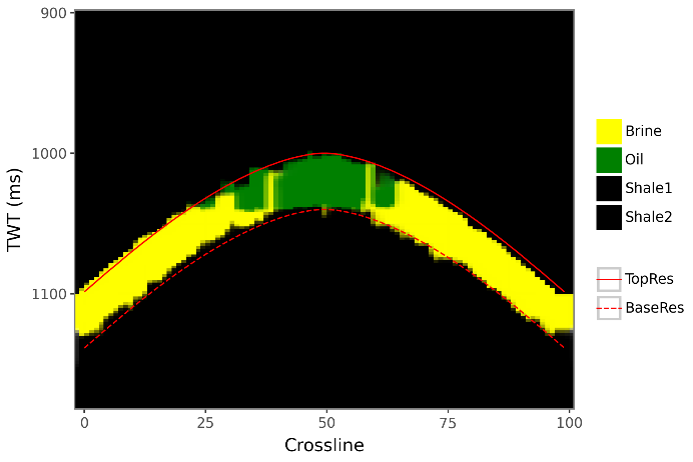
\includegraphics[width=0.8\textwidth]{figures/map_traces.png}
    \caption{Maximum a posteriori (MAP) traces for inline 50.}
    \label{fig:map_traces}
\end{figure}


\section{PCube GUI}

In this section we will describe the added functionality to the PCube standalone GUI.
The PCube tab MAP QC tab previously had support for inverting for elastic and reservoir
properties conditioned on the MAP QC tab. The tab now allows for a inverting for elastic
and reservoir properties conditioned on a custom user-specified LFC trace as well.
This allows for exploring different hypothesis and e.g. get at better understanding of the influence of the
LFC trace on the inverted properties. The custom LFC trace(s) may be imported from file,
either as a segy cube, or in text format. Please consult the User Manual for up to date
information. To reflect that we not only invert using the MAP trace, the tab has been renamed
\emph{Rock property inv. QC}.

\begin{figure}[h]
    \centering
    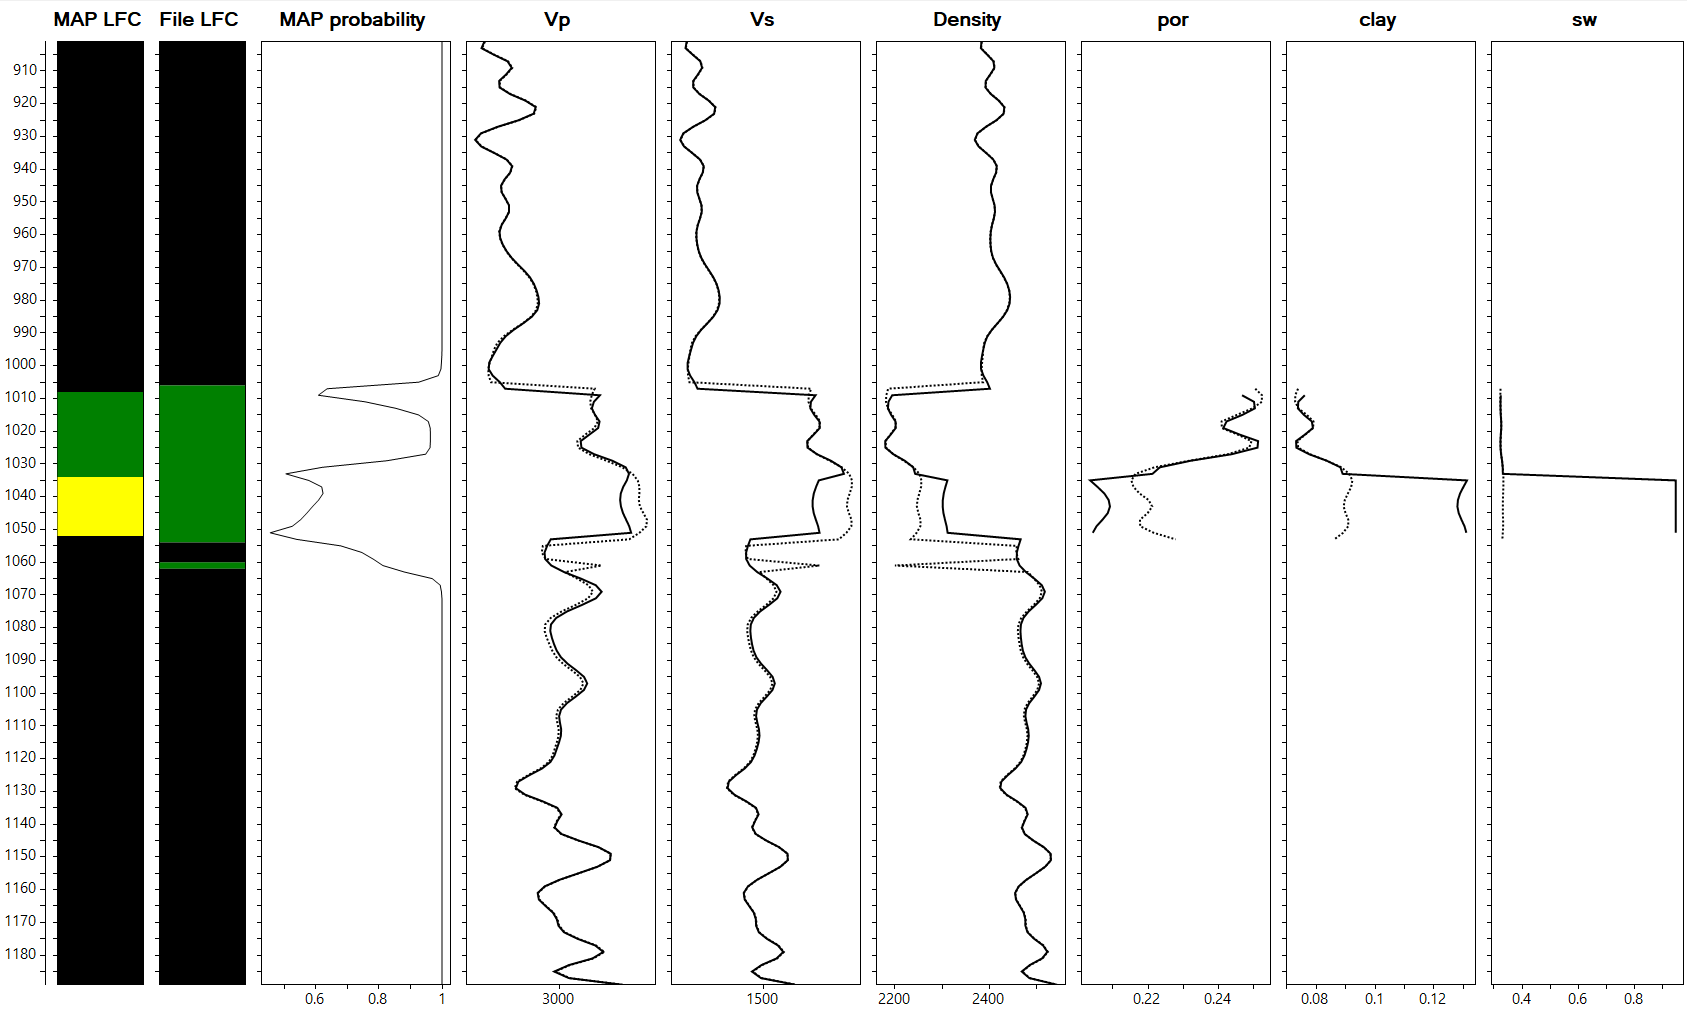
\includegraphics[width=\textwidth]{figures/gui_property_inversion_tab_il57_xl62_file.png}
    \caption{MAP LFC and custom LFC (from file) with inverted elastic and reservoir properties.
    The inverted properties for the MAP LFC are shown as solid lines, and
    the inverted properties for the custom LFC are shown as dotted lines.
    }
    \label{fig:custom_lfc_property_inversion_tab}
\end{figure}

In Figure \ref{fig:custom_lfc_property_inversion_tab} we show inverted properties
for a trace. Note that what is shown here is the posterior \textit{median} of the
properties. One might be interested in more than the just the median however, and
in the next section we shall see how we can both sample posterior properties,
as well as sampling LFC traces from the posterior Markov Chain for even more insight.

\section{Pycube module}

The goal of the new pycube module is twofold:
\begin{itemize}
    \item {
        Add more summaries and visualizations of inverted elastic and
        reservoir properties that can be easily generated from pycube.
        The added plots comes in the form of histograms, to view the
        full distribution of the data, or in form of maps, to visualize
        how the properties vary spatially.
    }
    \item{
        Add functionality in pycube to allow the user to easily estimate
        reservoir properties such as STOIIP and Net-to-Gross, that are not
        directly modeled in PCube, but can be estimated from
        other reservoir properties such as porosity and water saturation.
    }

\end{itemize}


It should be noted that the in PCube standalone we already have
the following outputs available in segy files:

\begin{itemize}
    \item Inverted median elastic and reservoir property cubes, as well as standard deviation.
    \item Histograms for individual elastic properties.
\end{itemize}

This information can also be generated from pycube when inverting a trace.
This module is a supplement to this functionality, and not a replacement.


\subsection{Example properties}
\label{sec:examples}

In Section \ref{sec:explanation} we will explain how the module works.
Before that we would like to show some examples of what you can
get out of the module, by showing a couple of reservoir
properties that could not previously be sampled, and how one
may configure the property inversion pycube module to achieve this.


\subsubsection{Hydrocarbon Pore Volume (HCPV)}

Estimating the amount of oil or gas in a reservoir is of course of great interest.
The Hydrocarbon Pore Volume (HCPV) is a common term used for the volume of the
hydrocarbons at reservoir conditions. Given the expansion factor of the hydrocarbons from the
reservoir to the surface, the HCPV can be converted to volume at surface
conditions, which is typically what is desired. Before production, in the
case of oil, this terms is known as STOIIP: Stock Tank Oil Initially-In-Place.
Here we concentrate on estimation of HCPV, modeling the expansion factor is out
of scope for this work.

The Hydrocarbon Pore Volume may be calculated as

\begin{equation}
HCPV = A * h * \phi * (1 - S_w)
\end{equation}

\begin{itemize}
    \item $A$ = Area in square meters.
    \item $h$ = Thickness in meters.
    \item $\phi$ = Porosity (fraction).
    \item $S_w$ = Water saturation (fraction).
\end{itemize}

In our calculations we will typically deviate from this definition in a few respects.
Firstly, we will typically calculate the HCPV on a trace basis, and only consider
the thickness, thus ignoring the area factor $A$. However, this should be easy to
multiply in as a postprocessing step.
Secondly, we don't necessarily try to calculate the total hydrocarbon
pore volume, but only the part that is economically recoverable. For example in areas
with high clay content or low porosity, we may choose to only include the net pay
in our calculations. This is configurable by the user.
Finally, we have the option to calculate the thickness in milliseconds as
well as in meters.


\begin{figure}[h]
    \centering
    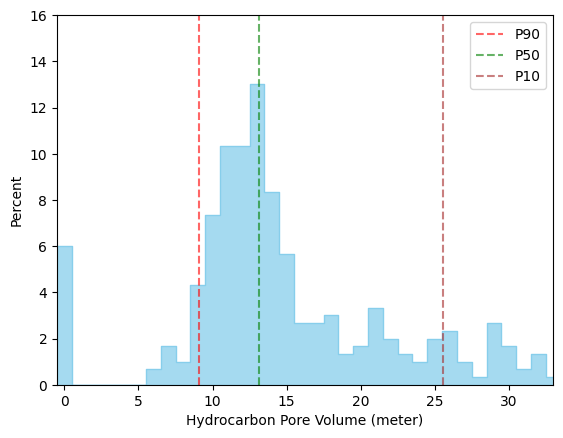
\includegraphics[width=0.8\textwidth]{figures/hydrocarbon_pore_volume_meters_il57_xl62.png}
    \caption{
        Histogram of sampled values of Hydrocarbon Pore Volume (HCPV) for inline $57$ and crossline $62$.
        We have also marked the P90, P50 and P10 values.
    }
    \label{fig:hydrocarbon_pore_volume}
\end{figure}


If Figure \ref{fig:hydrocarbon_pore_volume} we show a a histogram of sampled values of
HCPV for a single trace, and in Figure \ref{fig:hydrocarbon_pore_volume_maps} we show
P90, P50 and P10\footnote{The P90 value is the value for which 90 per cent of the
sampled value is at least as large as this value. P50 is the median, and only 10 per cent of the sampled values P10 or higher.} maps for
Hydrocarbon Pore Volume. We sampled $100$ LFC traces and $100$ properties for each
LFC trace, a total of $10000$ values for each inline and crossline location.
These are not $10000$ \textit{independent} samples however, see Section \ref{sec:sampling}.
We selected every other inline and
crossline to reduce compute time when generating the plots.

\begin{figure}[h]
    \centering
    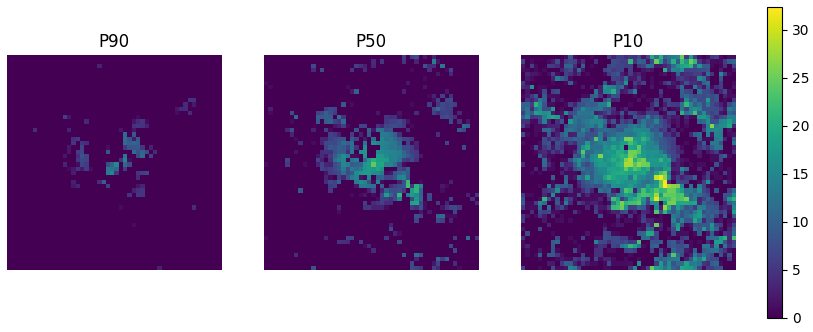
\includegraphics[width=\textwidth]{figures/hydrocarbon_pore_volume_meter_p90_p50_p10.png}
    \caption{P90, P50 and P10 maps of Hydrocarbon Pore Volume (HCPV) calculated in meters.}
    \label{fig:hydrocarbon_pore_volume_maps}
\end{figure}


\paragraph{Configuring HCPV}

Below we show how one may configure a property to calculate HCPV\footnote{
    All configurations are subject to change, refer to the latest PCube documentation.
}
\begin{minted}{yaml}
name: hydrocarbon_pore_volume
type: Thickness
config:
  lfcs: ["Oil"]
  property_criteria:
    - property: "por" # Porosity
      min_value: 0.2
    - property: "clay" # Clay fraction
      max_value: 0.1
  volume_factors:
    - property: "por"
    - property: "sw" # Water saturation
      use_complement: true # To get oil saturation (1 - sw)
  thickness_in_meters: true
\end{minted}

Let us go through the configuration in detail.
\begin{itemize}
    \item \emph{name}: Name of the property, can be chosen by the user.
    \item{\emph{type}: Type of property class to use, \emph{Thickness} in this case.}
    \item \emph{config}: Configuration parameters, for the Thickness property.
    \item \emph{lfcs}: List of LFCs which contain the hydrocarbon of interest.
    \item {
        \emph{property\_criteria}: This is optional, but here additional net pay criteria may be
        specified. Here we have specified two criteria. Having a minimum porosity of $0.2$
        and maximum clay content of $0.1$. Note that \textbf{por} and \textbf{clay} are the names
        of the porosity and clay reservoir properties respectively, and these must
        match the names given in the PCube project. If a sampled trace do not satisfy
        all of the criteria for parts of the trace, the parts that do not satisfy the
        criteria will not contribute to the hydrocarbon pore volume calculation.
    }
    \item {
        \emph{volume\_factors}: List of properties that we will multiply the
        net pay with in order to calculate HCPV. Here we specify that
        we should multiply with porosity, and one minus the water saturation,
        as the use complement flag is specified here.
    }
    \item \emph{thickness\_in\_meters}: If true we calculate the thickness in meters, otherwise in milliseconds.
\end{itemize}

If we try to connect the configuration to the original HCPV definition, we
have that LFCs and property criteria determines $h$ (and the \emph{thickness\_in\_meters}
parameter determine if this is in meters or milliseconds), while
the volume factors specify the $\phi$ and $(1 - S_w)$ terms.

\subsubsection{Net-to-Gross (NTG)}

Net-to-Gross is another property that may be of interest in determining
productive zones in a reservoir.
We try to be as flexible as possible to allow for different ways of
defining how it should be calculated.

If Figure \ref{fig:net_to_gross_histogram} we show an example of a histogram
of sampled net-to-gross values for a single trace.
\begin{figure}[h]
    \centering
    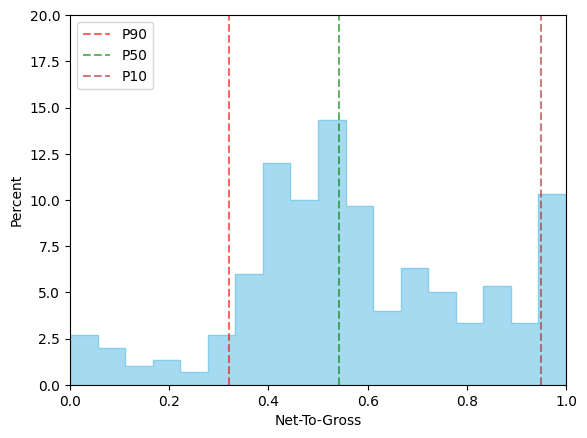
\includegraphics[width=0.8\textwidth]{figures/net_to_gross_il57_xl62.png}
    \caption{Histogram of sampled values of Net-to-Gross for inline $57$ and crossline $62$.}
    \label{fig:net_to_gross_histogram}
\end{figure}


In Figure \ref{fig:net_to_gross_maps} we show P10, P50 and P90 maps for
Net-to-Gross. For each inline and crossline we use the same sampled lfc
traces and properties that we used to calculate the Hydrocarbon Pore Volume

\begin{figure}[h]
    \centering
    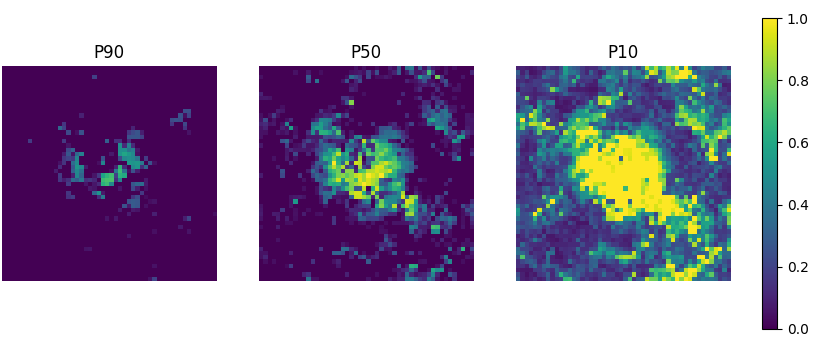
\includegraphics[width=\textwidth]{figures/net_to_gross_p90_p50_p10.png}
    \caption{P90, P50 and P10 maps of Net-to-Gross.}
    \label{fig:net_to_gross_maps}
\end{figure}


\paragraph{Configuring Net-to-Gross}

Below we show how one may configure a property to calculate Net-to-Gross.
\begin{minted}{yaml}
name: net_to_gross
type: NetToGross
config:
  lfcs_gross: ["Oil", "Brine"]
  lfcs_net: ["Oil"]
  property_criteria:
    - property: "por"
      min_value: 0.2
    - property: "clay"
      max_value: 0.1
  thickness_in_meters: false
\end{minted}

Let us go through the configuration.
\begin{itemize}
    \item \emph{name}: Name of the property, can be chosen by the user.
    \item{\emph{type}: Type of property class to use, here \emph{NetToGross}}
    \item \emph{config}: Configuration parameters, for the NetToGross property.
    \item \emph{lfcs\_gross}: List of lfcs for gross pay. Here we include both oil and brine saturated sandstones.
    \item \emph{lfcs\_net}: List of lfc names to include in net pay, here only oil sand is counted.
    \item {
        \emph{property\_criteria}: Additional Net Pay criteria may be
        specified. Here we have specified the same criteria as for HCPV,
        having a minimum porosity of $0.2$ and maximum clay proportion of $0.1$.
    }
    \item {
        \emph{thickness\_in\_meters}: If true we calculate the thickness of net and gross
        pay in meters before taking the ratio.
    }
\end{itemize}


\subsection{Explanation of process}
\label{sec:explanation}

In this section we will explain the steps in how we sample from the
posterior distribution for elastic and reservoir properties.

\subsubsection{Sample LFC traces}

\begin{figure}[htbp]
    \begin{minipage}[valign=t]{0.9\textwidth}
        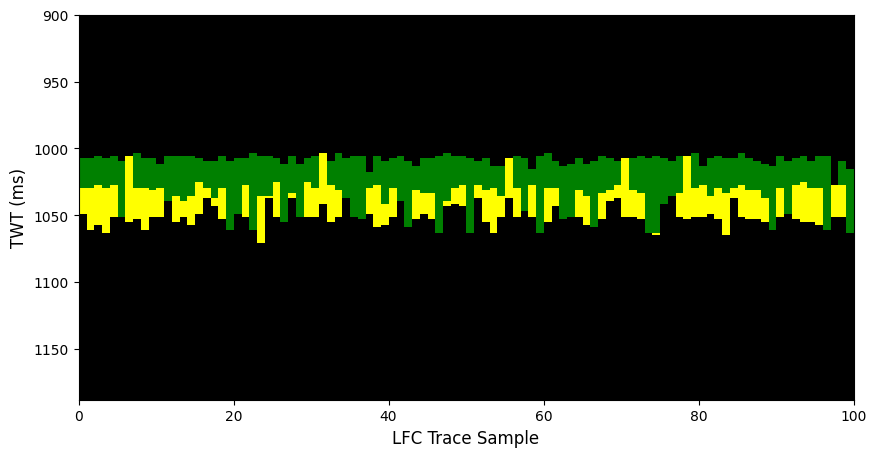
\includegraphics[width=\textwidth]{figures/lfc_traces_sampled_il57_xl62.png}
    \end{minipage}%
    \begin{minipage}[valign=t]{0.1\textwidth}
        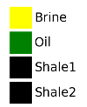
\includegraphics[width=\textwidth]{figures/lfc_legend.png}
    \end{minipage}
    \caption{$100$ LFC traces samples from posterior Markov Chain.
             Each vertical slice is an independently sampled LFC trace.
    }
    \label{fig:lfc_traces}
\end{figure}

The first step is to sample LFC traces from the posterior Markov Chain.
In Figure \ref{fig:lfc_traces} we show
sampled LFC traces for a given trace location.

The number of LFC samples per trace is configurable.

\subsubsection{Sample elastic and reservoir properties}
For each LFC trace we then sample elastic and reservoir properties
from the posterior distribution, given the data and LFC trace.
The number of samples here is also configurable. In Figure \ref{fig:sampled_properties}
we show three samples of elastic and reservoir properties for a given LFC trace. Note that
for a given sample, we use the joint posterior distribution of all elastics
and reservoir properties.
\begin{figure}[h]
    \centering
    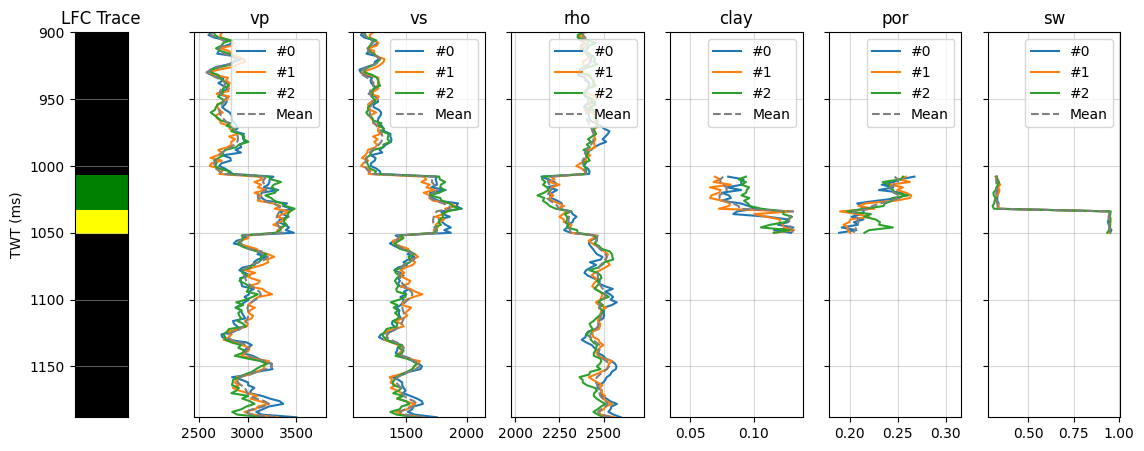
\includegraphics[width=\textwidth]{figures/sampled_properties_with_mean_il57_xl62.png}
    \caption{Three samples of reservoir properties for a given LFC trace. The posterior median is shown as a dotted line.}
    \label{fig:sampled_properties}
\end{figure}

The number of elastic and reservoir property samples per LFC trace is configurable.

\subsubsection{Calculate properties of interest}

\begin{figure}[h]
    \centering
    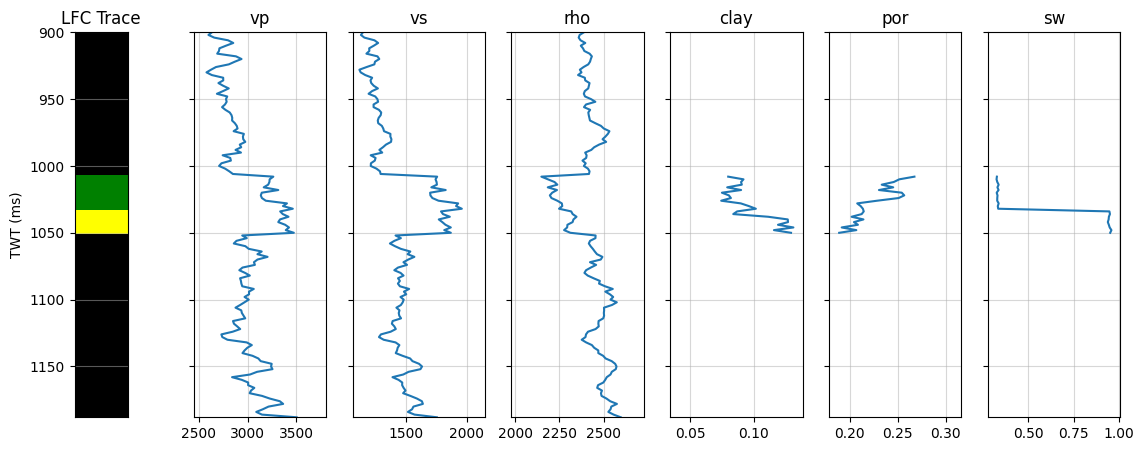
\includegraphics[width=\textwidth]{figures/sampled_properties_il57_xl62.png}
    \caption{LFC trace with properties sampled from posterior distribution.}
    \label{fig:lfc_trace_and_properties}
\end{figure}

Until now we have described the sampling machinery, now we come to the arguably
more interesting part. In Figure \ref{fig:lfc_trace_and_properties} we show an
example of a LFC trace together with sampled properties. Together this is considered
a single sample from our posterior distribution. Based on this sample we may
now calculate a property of interest. This may be HCPV, Net-to-Gross or any
other property of desire. We have shown examples of this in Section \ref{sec:examples}.

The only restriction of a property is that given an LFC-trace and a set of
properties, it should produce a \textit{single} number or boolean value.
In other words, we should not produce one value for each depth level,
but one value for the entire trace. This fits very well with our example properties,
which are based on based on thickness in the case of HCPV or comparisons of
thicknesses in the case of Net-To-Gross. An example of a boolean property
could be e.g. a property that returned true if the sampled trace contained
net pay, otherwise false.

Notice the similarities of Figure \ref{fig:lfc_trace_and_properties} and
Figure \ref{fig:custom_lfc_property_inversion_tab}. There are however two
crucial differences:
\begin{itemize}
    \item In the GUI tab the LFC trace is either the MAP LFC or a custom LFC trace
          from the user, while in the pycube module we sample LFC traces
          from the posterior Markov Chain.
    \item In the GUI tab we show the posterior \textit{median} of the properties,
          while in the pycube module we \textit{sample} properties from the posterior
          distribution given the LFC trace.
\end{itemize}

The module establishes a common framework for estimating any property that
is based on the elastic and reservoir properties. The module handles all the
sampling and book keeping. In the case of a 4D project the properties will
be split into base and monitor after sampling, and the property will be
evaluated separately for each vintage.

In section \ref{sec:examples} we covered configuration of Hydrocarbon Pore
Volume and Net-to-Gross properties. In general each property type will
have their own configuration options, so consult the module documentation
for up-to-date information.

\subsubsection{Visualize}

We support two types of visualizations out of the box.

\begin{itemize}
    \item Histogram of the full distribution of a property.
    \item Maps, mean map or e.g. P10, P50, P90 maps of the property of interest.
\end{itemize}

Note that the sampled custom properties may be written to a \emph{csv}
or \emph{parquet} file as well. This has the advantage of both access to the
data used in generating the plots, as well as the ability to
fine tune plots or create completely new visualizations.

\paragraph{Configuring Visualization}

Here is an example configuration for the visualizations:
\begin{minted}{yaml}
summaries_config:
  - type: MeanMap
    config: {}
  - type: PercentileMaps
    config:
      percentiles: [90, 50, 10]
  - type: Histogram
    config:
      ignore_zero: true
\end{minted}


Let us go through the configuration:
\begin{itemize}
    \item{
        \emph{summaries\_config}: List of summaries to generate for each property.
    }
    \item{
        \emph{type}: Type of summary to generate. Here we have three types:
        MeanMap, PercentileMaps and Histogram.
    }
    \item{
        \emph{config}: Configuration parameters for the summary type.
    }
    \item{
        The \emph{MeanMap} do not have any required configuration parameters.
    }
    \item{
        The \emph{PercentileMaps} have the following configuration parameters:
        \begin{itemize}
            \item \emph{percentiles}: List of percentiles to generate maps for.
        \end{itemize}
    }
    \item{
        The \emph{Histogram} have the following configuration parameters:
        \begin{itemize}
            \item \emph{ignore\_zero}: If true, zero values are ignored when generating the histogram.
              This may be useful if the property of interest is zero in large parts of the model,
              as this may dominate the histogram.
        \end{itemize}
    }
\end{itemize}

Note that each property type may be specified several times with different configurations.
One may e.g. use the Thickness property to estimate both gross and net pay,
or have two versions of the same property, one in meters and one in milliseconds.

\subsubsection{Note on sampling}
\label{sec:sampling}

If we sample $100$ LFC traces and sample $100$ sets of properties for each
LFC sample we have $10000$ realizations of property values from the posterior distribution.
Note however that we don't have $10000$
\textit{independent} samples, as samples that condition on the same LFC
trace will not be independent. If we instead only drew $1$ property sample per LFC trace
all samples would be independent. This would however come at the cost of either fewer
samples or increased compute time, as the most time consuming part of the inversion
is to find posterior mean and covariance (in transformed domain) given an LFC trace.
Sampling many properties given that posterior mean and covariance is comparably cheap.
One way to think about it is that we get $100$ independent samples, one for each LFC trace, and then we
get some additional dependent samples. Though these do not give the same benefit
as fully independent samples, it can be justified by their cheap calculation.
As an analogy, assume you want to find the expectation of a random variable by taking
the average of a sample for the distribution. It is better to have $10$ samples then
$1$, as long as they are not perfectly correlated. The lower the correlation is, the
more is the variance of the estimator is reduced.

Note that we may split the variance that is explained by the variation in LFC traces,
and the variation that is due to property sampling. By the law of total variance
the variance of a random variable $Y$ we have

It should be noted that for cases with low variation in the reservoir properties,
most of the variation may be attributed to LFC thickness only. In these cases one may get
a much faster estimate of HPCV by only sampling LFC traces from the posterior Markov Chain,
and not inverting for elastics and reservoir properties, and just use constant values for these.
In this case one may generate this data when running PCube inversion by specifying this
in the PCube output configuration.

\begin{align*}
\text{Var}(Y) &= \text{Var}(\mathbb{E}[Y | X]) + \mathbb{E}[\text{Var}(Y | X)]
\end{align*}

e.g. for the Hydrocarbon Pore Volume we may write this as

\begin{align*}
\text{Var}(\text{HCPV}) &= \text{Var}(\mathbb{E}[\text{HCPV} | \text{LFC}]) + \mathbb{E}[\text{Var}(\text{HCPV} | \text{LFC})]
\end{align*}

The first part is due the variance in LFC traces, while the second part
is the variance in property sampling. Assume now we want to estimate the
mean of the property. By increasing the number of property
samples per LFC trace we may reduce the second term as much as we desire,
but we need to increase the number of LFC samples to reduce the first term.


\subsection{Python implementation}

Here we show an outline of the abstract \emph{CustomProperty} class with
two methods that needs to be implemented by all custom properties (which
should extend this class).

\begin{minted}{python}

class CustomProperty(abc.ABC):
    # ...
    def lfc_names(self) -> list[str]:
        """List of LFC names used for this custom property."""
        raise NotImplementedError(
            "This method should be overridden in subclasses to return the LFC indices."
        )

    def evaluate_property(properties: dict[str, np.ndarray]) -> float | int | bool:
        """Evaluate the custom property based on the provided elastic and reservoir properties.

        Args:
            properties (dict[str, np.ndarray]): Dictionary of properties where
              keys are property names (elastic or reservoir) and values are numpy arrays
              of property values. The properties provided are the ones specified in
              `input_properties`.
        Returns:
            Evaluated custom property value, should be a scalar.
        """
        raise NotImplementedError(
            "This method should be overridden in subclasses to evaluate the custom property."
        )
\end{minted}

The \emph{lfc\_names} function should return a list of LFC names. The
names are used to filter the trace to only the part of the
trace of the LFCs of interest.

The \emph{evaluate\_property} function takes as input a set of sample properties

As part of this work package we have implemented three custom properties:
\begin{itemize}
    \item \emph{Thickness} can be configured to calculate e.g. hydrocarbon pore volume, gross pay or net pay.
    \item \emph{NetToGross} is used to calculate Net-to-Gross.
    \item \emph{PresenceProbability} Can be configured to e.g. calculate the probability of hydrocarbon presence or net pay presence.
\end{itemize}


\section{Summary}
In this note we have described a new property inversion module in pycube.
The module is flexible and can be configured from yaml files. The property
inversion can be quite computationally demanding, however, so it is
recommended to first narrow down the area of interest to keep computation
time reasonable.

\bibliography{references.bib}
\end{document}
